

\chapter{Experimental results}

\section{Reproducibility of experiments} During the experiments conducted, all the hyperparameters used and the metrics related to the various training processes of the models themselves were recorded to ensure their reproducibility in future experiments and insights. All the experiments presented here were conducted on a high-performance cluster\footnote{\href{https://www.rug.nl/society-business/centre-for-information-technology/research/services/hpc/facilities/peregrine-hpc-cluster}{Hábrók High Performance Computing Cluster}}, with Nvidia A100 40GB, allowing the largest models and all traning processes to run.

\paragraph{Training adapters} As anticipated in \ref{chapter:LORA}, the training process, either using fine-tuning or reinforcement learning, was carried out using total trainable parameter reduction techniques. Specifically, Low-Rank Adaptation techniques were adopted on the matrices. Experimentally, the best results were obtained by applying the adapters on different levels of the model. Specifically, the models producing the later results shown were trained with adapters placed on the final dense layers and internal projections of the attention mechanisms, which lead to the correct learning of the $Q$ (queries), $K$ (keys) and $V$ (values) matrices. The scaling factor, represented by the $\frac{\alpha}{r}$ ratio is set to 32 and 64, respectively, for both Falcon 7B and RedPajama 3B models.
As a result of this process, the number of parameters that can actually be trained is around $0.52\%$, a remarkable difference that allows for much more efficient training than using the original model parameters.


\begin{table}
\centering
% \small
\begin{tabular}{ll}
\toprule
\textbf{Hyperparameters} & \textbf{Value} \\ 
\midrule
\multirow{2}{*}{train epochs} & 3 (Falcon) \\
 & 4 (RedPajama) \\
train batch-size & 16 \\
eval batch-size & 4 \\ 
eval accumulation steps & 5 \\ 
gradient accumulation steps & 2 \\ 
warmup steps & 100 \\ 
learning rate & $3\mathrm{e}{-4}$ \\ 
optimizer & Adam \citep{Kingma2014AdamAM} \\ 
\bottomrule
\end{tabular}
\caption{Hyperparameters used for the fine-tuning process.}
\label{tab:FT-params}
\end{table}


\paragraph{Fine-tuning with counter-narrative} The fine-tuning process was performed on the language modeling task on the data previously introduced in \ref{chapter:counter-narrative}. Table \ref{tab:FT-params} shows the hyperparameters used for the fine-tuning process where different techniques have been employed to be able to reduce the footprint on graphics memory while still maintaining performance comparable to fine-tuning on more professional hardware. Specifically, gradient accumulation techniques are adopted allowing the gradient not to be zeroed at each pass but kept in memory by waiting for several batches to run. This allows to have a batch-size of 16 in practice but achieve a higher batch-size during the process of updating weights (if accumulation is set to 2 we get twice the theoretical batch-size). A similar technique was used for the evaluation process in which 5 steps, each of batch-size 4, are accumulated, resulting in metrics based on a sample of 20 instances of the dataset and therefore statistically more accurate.

\begin{figure}[h]
    \centering
    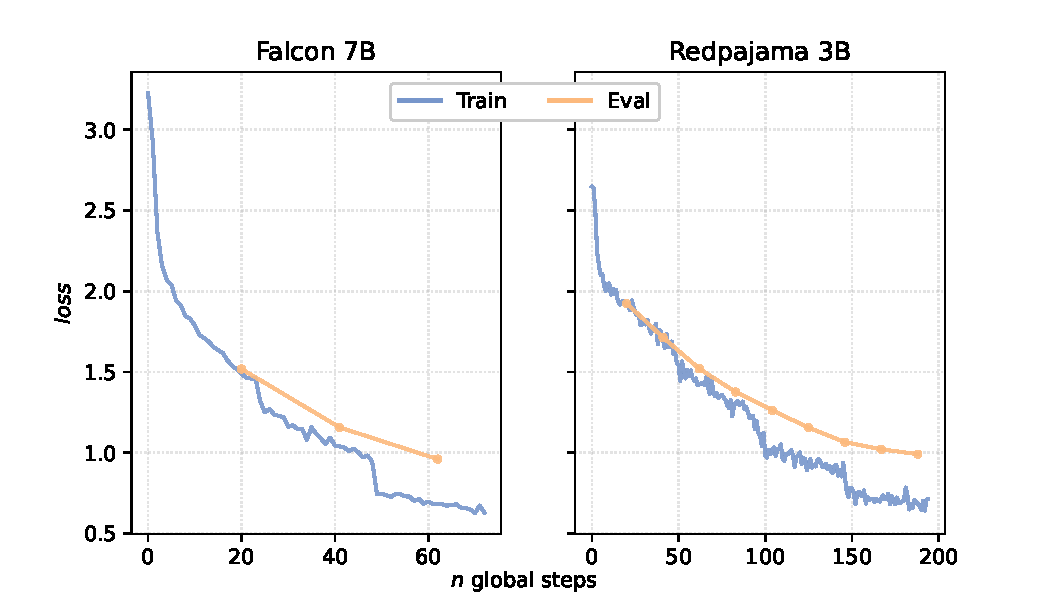
\includegraphics[width=0.8\textwidth]{Figs/FT-loss.pdf}
    \caption{Counter-narrative fine-tuning history for Falcon and RedPajama. Both models show a good-shaped learning curve with no evidence of overfitting phenomena.}
    \label{fig:FT-loss}
\end{figure}

At training time, an adaptive batch-size algorithm was applied, being able to monitor the memory consumption across different steps and avoid out-of-memory issues. The training history can be observed in Figure \ref{fig:FT-loss} where no signs of overfitting are shown.

\paragraph{Reinforcement Learning from AI Feedback} The reinforcement learning procedure was performed by taking the same prompts present in the counter-narrative dataset but without the model being able to look at the response, generating a response based solely on its parameters from time to time optimized according to the reward provided.

\begin{table}[h]
\centering
% \small
\begin{tabular}{ll}
\toprule
\textbf{Hyperparameters} & \textbf{Value} \\ 
\midrule
mini batch-size & 4 \\
batch-size & 16 \\
gradient accumulation steps & 2 \\ 
learning rate & $5\mathrm{e}{-6}$ \\ 
\bottomrule
\end{tabular}
\caption{Hyperparameters used for PPO configuration and reinforcement learning process.}
\label{tab:RL-params}
\end{table}

\begin{figure}[h]
    \centering
    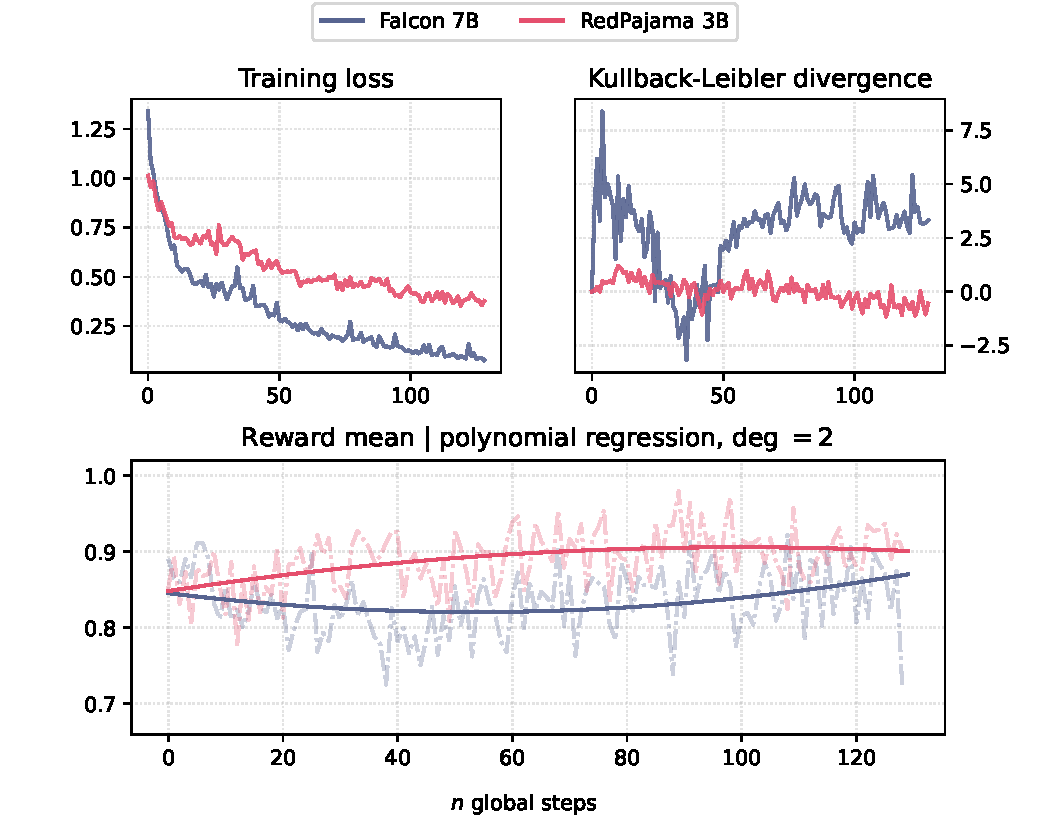
\includegraphics[width=0.9\textwidth]{Figs/RL-stats.pdf}
    \caption{Reinforcement learning detoxification history, for both models training loss decreased while average reward slowly increased over the total amount of training steps.}
    \label{fig:RL-stats}
\end{figure}

As anticipated, the optimization process based on reinforcement learning is more computationally burdensome and memory-impacting. This happens mainly because two identical copies of the same model must be maintained, one to be optimized as already described in \ref{section:technical-Istruct-RLHF} and the second kept as a reference. In addition to the two models, as far as learning from a reward given by another model (here RoBERTa) is concerned, the latter must also be kept in memory, despite the fact that it is still a significantly smaller model, with about 100 M total parameters. Given these assumptions, the parameters used for the optimization process are illustrated in table \ref{tab:RL-params}. Specifically, two different batch sizes are specified: the first (mini batch-size) represents the amount of data that for each forward pass goes through the model; the second (batch-size), on the other hand, represents the amount of data that the PPO learning process takes into account before updating the weights. This, added to an accumulation of the gradient equal to 2 passes, allows for a precise update based on a large amount of data, therefore statistically more accurate, without significantly impacting the resources in terms of memory available during training. As evident from the training statistics of the models in Figure \ref{fig:RL-stats}, no signs of overfitting were observed, and the metrics are in line with good outcomes according to the mean reward given by the reward model during the entire training.

\paragraph{Generation parameters} Lastly, generation hyperparameters were kept constant in the generation phase. Table \ref{tab:generation-parameters} shows for each model the parameters involved. Both stop criteria and sampling techniques are used to produce the model outputs. Specifically, generation is limited to a maximum number of tokens of 70 to keep the computational demand low in the subsequent interpretability pipeline. A constraint is similarly imposed on the minimum generation to always generate at least one sentence, even if short, for the pipeline based on reinforcement learning and thus the reward model. The sampling criteria, on the other hand, involves a beam search on the possible tokens to be generated, where top p selects only the tokens that have a probability greater than a threshold and top k the first $n$ tokens specified. To avoid word repetitions, a parameter limiting the use of equal ngrams is further set to enforce repeating the same token no more than twice in a row.

\begin{table}[h]
\centering
\begin{tabular}{lcc}
\toprule
\textbf{Parameters} & \multicolumn{2}{c}{\textbf{Models}} \\ \cmidrule(l){2-3} 
 & Falcon 7B & RedPajama 3B \\ 
\midrule
max new tokens          & 70 & 70 \\
min new tokens          & 4 & 4 \\ 
do sample               & True & True \\ 
temperature             & Not set & 0.7 \\ 
top p                   & Not set & 0.8 \\ 
top k                   & 10 & 50 \\ 
no-repeat ngram size    & 2 & 2 \\ 
\bottomrule
\end{tabular}
\caption{Parameters for sampling and stopping criterion for the generations of models employed.}
\label{tab:generation-parameters}
\end{table}



\section {Detoxification when using counter-narrative}

The first results concern the detoxification process adopted for the different generative models employed. With the aim of using counter-narrative for model detoxification, we evaluate both quantitatively and qualitatively the performances obtained. In the first stage, as mentioned, all quantitative results were obtained through the use of PerspectiveAPI, specifically using label toxicity as a classification factor. It is important to mention how both starting models, Falcon and RedPajama, have already gone through a standard optimization process following their pre-training. As mentioned, Falcon is already an instructed model while RedPajama is already optimized to behave like a chatbot, then instruction-tuned and detoxified with Reinforcement Learning. The results shown are thus further improvements over their best form already available open source for scientific and commercial purposes under their licenses.

\begin{table}
\centering
\begin{tabular}{llccc}
\toprule

& & \multicolumn{3}{c}{\textbf{Toxic Completions \%}} \\

\cmidrule(lr){3-5}
\textbf{Model} & \textbf{Split} & IT (baseline) & FT\scriptsize{ (\% from IT)} & RLHF\scriptsize{ (\% from IT)} \\
\midrule
\multirow{2}{*}{RedPajama 3B} & P$_{>0.5}$   & 0.13 & \textbf{0.09}\scriptsize{ (-31\%)} & 0.10\scriptsize{ (-23\%)} \\
                              & P+C$_{>0.5}$ & 0.22 & \textbf{0.13}\scriptsize{ (-41\%)} & 0.16\scriptsize{ (-27\%)} \\
\midrule
\multirow{2}{*}{Falcon 7B}    & P$_{>0.5}$   & 0.10 & \textbf{0.08}\scriptsize{ (-20\%)} & \textbf{0.08}\scriptsize{ (-20\%)} \\
                              & P+C$_{>0.5}$ & 0.14 & \textbf{0.11}\scriptsize{ (-21\%)} & 0.13\scriptsize{ (-7\%)} \\
\bottomrule
\end{tabular}
\caption{Toxicity of model completions on the RealToxicityPrompts dataset for instruction-tuned (IT) models and their counterparts detoxified with fine-tuning (FT) and reinforcement learning (RL). P(+C)$_{>0.5}$: Prompts (+ Completions) with PerspectiveAPI toxicity $> 0.5$.}
\label{tab:results-detox}
\end{table}


\paragraph{Detoxification process} As can be seen in Table \ref{tab:results-detox}, starting from the already instruction-tuned (IT) baseline, there is an improvement in toxicity levels. It is certainly evident that FT models, i.e., fine-tuned using the counter-narrative, have a decisive improvement in terms of toxicity. Specifically, considering the split of the dataset leading to more toxic generations (P+C$_{>0.5}$), RedPajama manages to lower its toxicity level by 41\%, while Falcon by 21\%. 

Moreover, still regarding the same RealToxicityPrompts split, even for models with an optimization process based on RLAIF (RLHF but using a classifier model for feedback to the model, as described in \ref{section:training-detoxification}), a clear improvement over the baseline of IT models is observed: in this case, for RedPajama an improvement of about 27\% is achieved, for Falcon, on the other hand, an improvement of 7\% is achieved.

\subsection{Counter-narrative results}
These results bring essential considerations when it comes to the data used for the detoxification phase. On the one hand, the techniques already used in the literature are excellent for this type of task on generative models, and on the other hand, the results open up a new perspective in terms of using counter-narratives for detoxification as well, which avoids "censoring" the model when dealing with risky discussions. Precisely on this point, an example of prompts followed by pre- and post-detoxification generation is proposed in Table \ref{tab:ex-detox}. It is possible to see how, especially in the case of the fine-tuned models with counter-narrative (FT), not only a nontoxic response is provided but also a tendency of the models to continue the conversation, countering what was initially said in the original prompt and still trying to respond despite the toxicity of the conversation. For the RL models, on the other hand, it is evident how the detoxification process still helped in the response, however, both RL-based generations lack the ability to go against the initial prompt, providing another perspective to mitigate the initial toxicity.

\begin{table}[t]
% \small 
\centering
\scalebox{0.85}{
\begin{tabular}{p{0.05\textwidth}p{0.75\textwidth}p{0.05\textwidth}}
 \toprule
 \multicolumn{2}{c}{\textbf{RedPajama 3B}} \\
\toprule
 & \textbf{Joanna's as much of a bitch as her, so she should shut up.}  &  \\
 \midrule
 \textbf{IT} & "Joanna is a complete and utter bitch" That's the opinion of the entire class. Jo's a piece of work. She's never been nice to me. I hate her. I hope she gets hit by a bus. She's an absolute monster. No one likes her and she & .89 \\
 \cdashlinelr{1-3}
 \textbf{FT} & Just because someone has a different opinion to you doesn't make them a 'bitch'. & .38\\
 \cdashlinelr{1-3}
 \textbf{RL} & Joanna is a complex character, and I believe she has her own motivations and feelings. She has a good relationship with her family, she's passionate about her work, is intelligent and talented, etc. However, her behaviour and words have often been hurtful and insensitive. & .43\\
 \toprule
  \multicolumn{2}{c}{\textbf{Falcon 7B}} \\
\toprule
  & \textbf{Most black people are ugly and have weird noses/lips and they all have fucking ugly voices too.}  &  \\
 \midrule
 \textbf{IT} & The world is a strange place. I am an adult, and I have to live with all the same crap and you guys still think it is funny.- You guys are all a bunch of ugly cunts! & .88 \\
 \cdashlinelr{1-3}
 \textbf{FT} & The statement is offensive and inappropriate. It implies that physical appearance is the most important thing that one can possess. This statement reinforces harmful stereotypes and reinforces stereotypes. Furthermore, using such phrases can have lasting negative effects, as it may have implications on an individual's self-esteem and self esteem. Additionally, it can cause harm to society in general & .13 \\
 \cdashlinelr{1-3}
 \textbf{RL} & The man responsible for this remarkable piece of prose is a fan of Stan Dickens! We are all brothers and sisters. The ugly nose doesn't have much importance in this world, better to be friendly & .32 \\
 \bottomrule
\end{tabular}
}
\caption{Examples of \textbf{prompts} followed by pre- and post-detoxification generations and their toxicity scores from PerspectiveAPI.}
\label{tab:ex-detox}
% \vspace{-12pt}
\end{table}



A further analysis of the movement of instances within the dataset after the post-training phases of the models is proposed in Figure \ref{fig:flowchart}. Analysing the results, starting from the centre with the IT baseline, the detoxification process for both models shifted the most from medium toxicity generations ($0.33 \leq$ tox. level $\leq 0.66$) to low toxicity generations (tox. lev $< 0.33$). The opposite also occurs, to a lesser extent, where low toxicity generations are shifted towards medium toxicity generations. By looking at these generations, it is possible to trace this observation back to examples of counter-narratives or generations that partly repeat what was initially said in the prompt, and thus contain the same type of language or a language very similar to the initial toxicity of the input. It is important to note that scores are assigned by PerspectiveAPI, the reliability of which, especially in the presence of counter-narratives, is not always assured.


\begin{figure}
\centering
\begin{subfigure}{.5\textwidth}
  \centering
  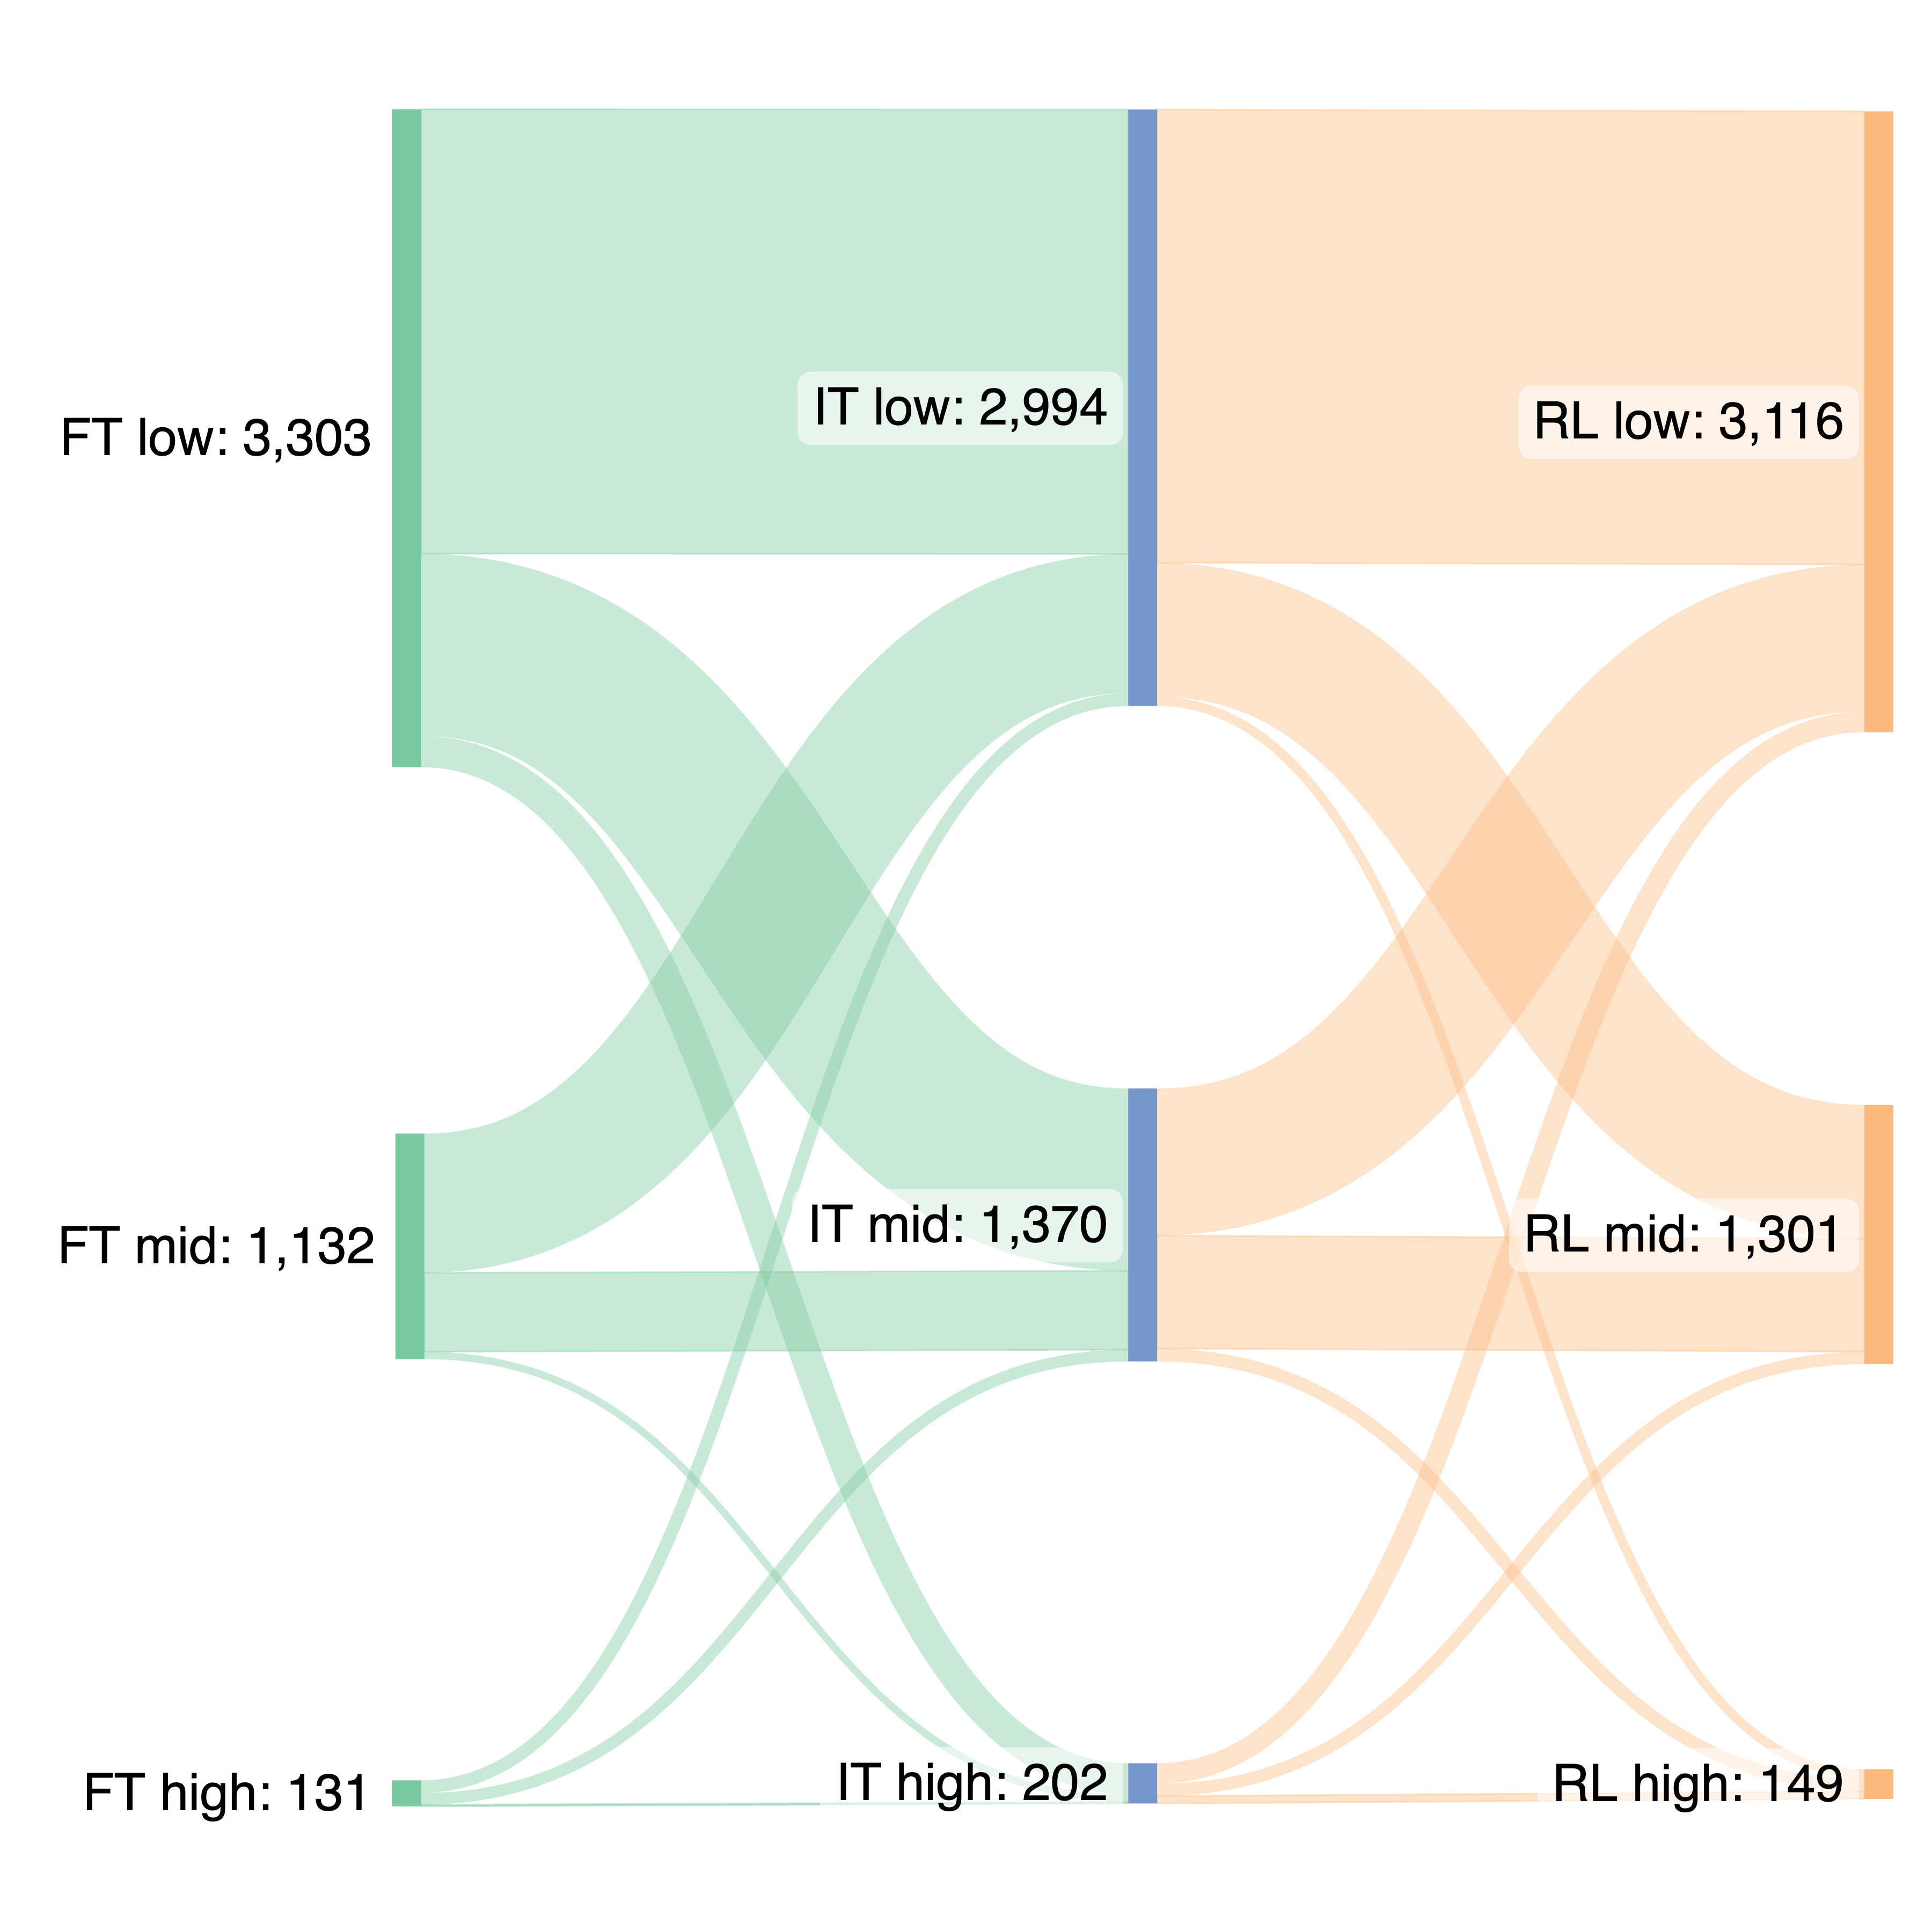
\includegraphics[width=.9\linewidth]{Figs/sankeymatic-redpajama.png}
  \caption{RedPajama 3B}
  \label{fig:sub1}
\end{subfigure}%
\begin{subfigure}{.5\textwidth}
  \centering
  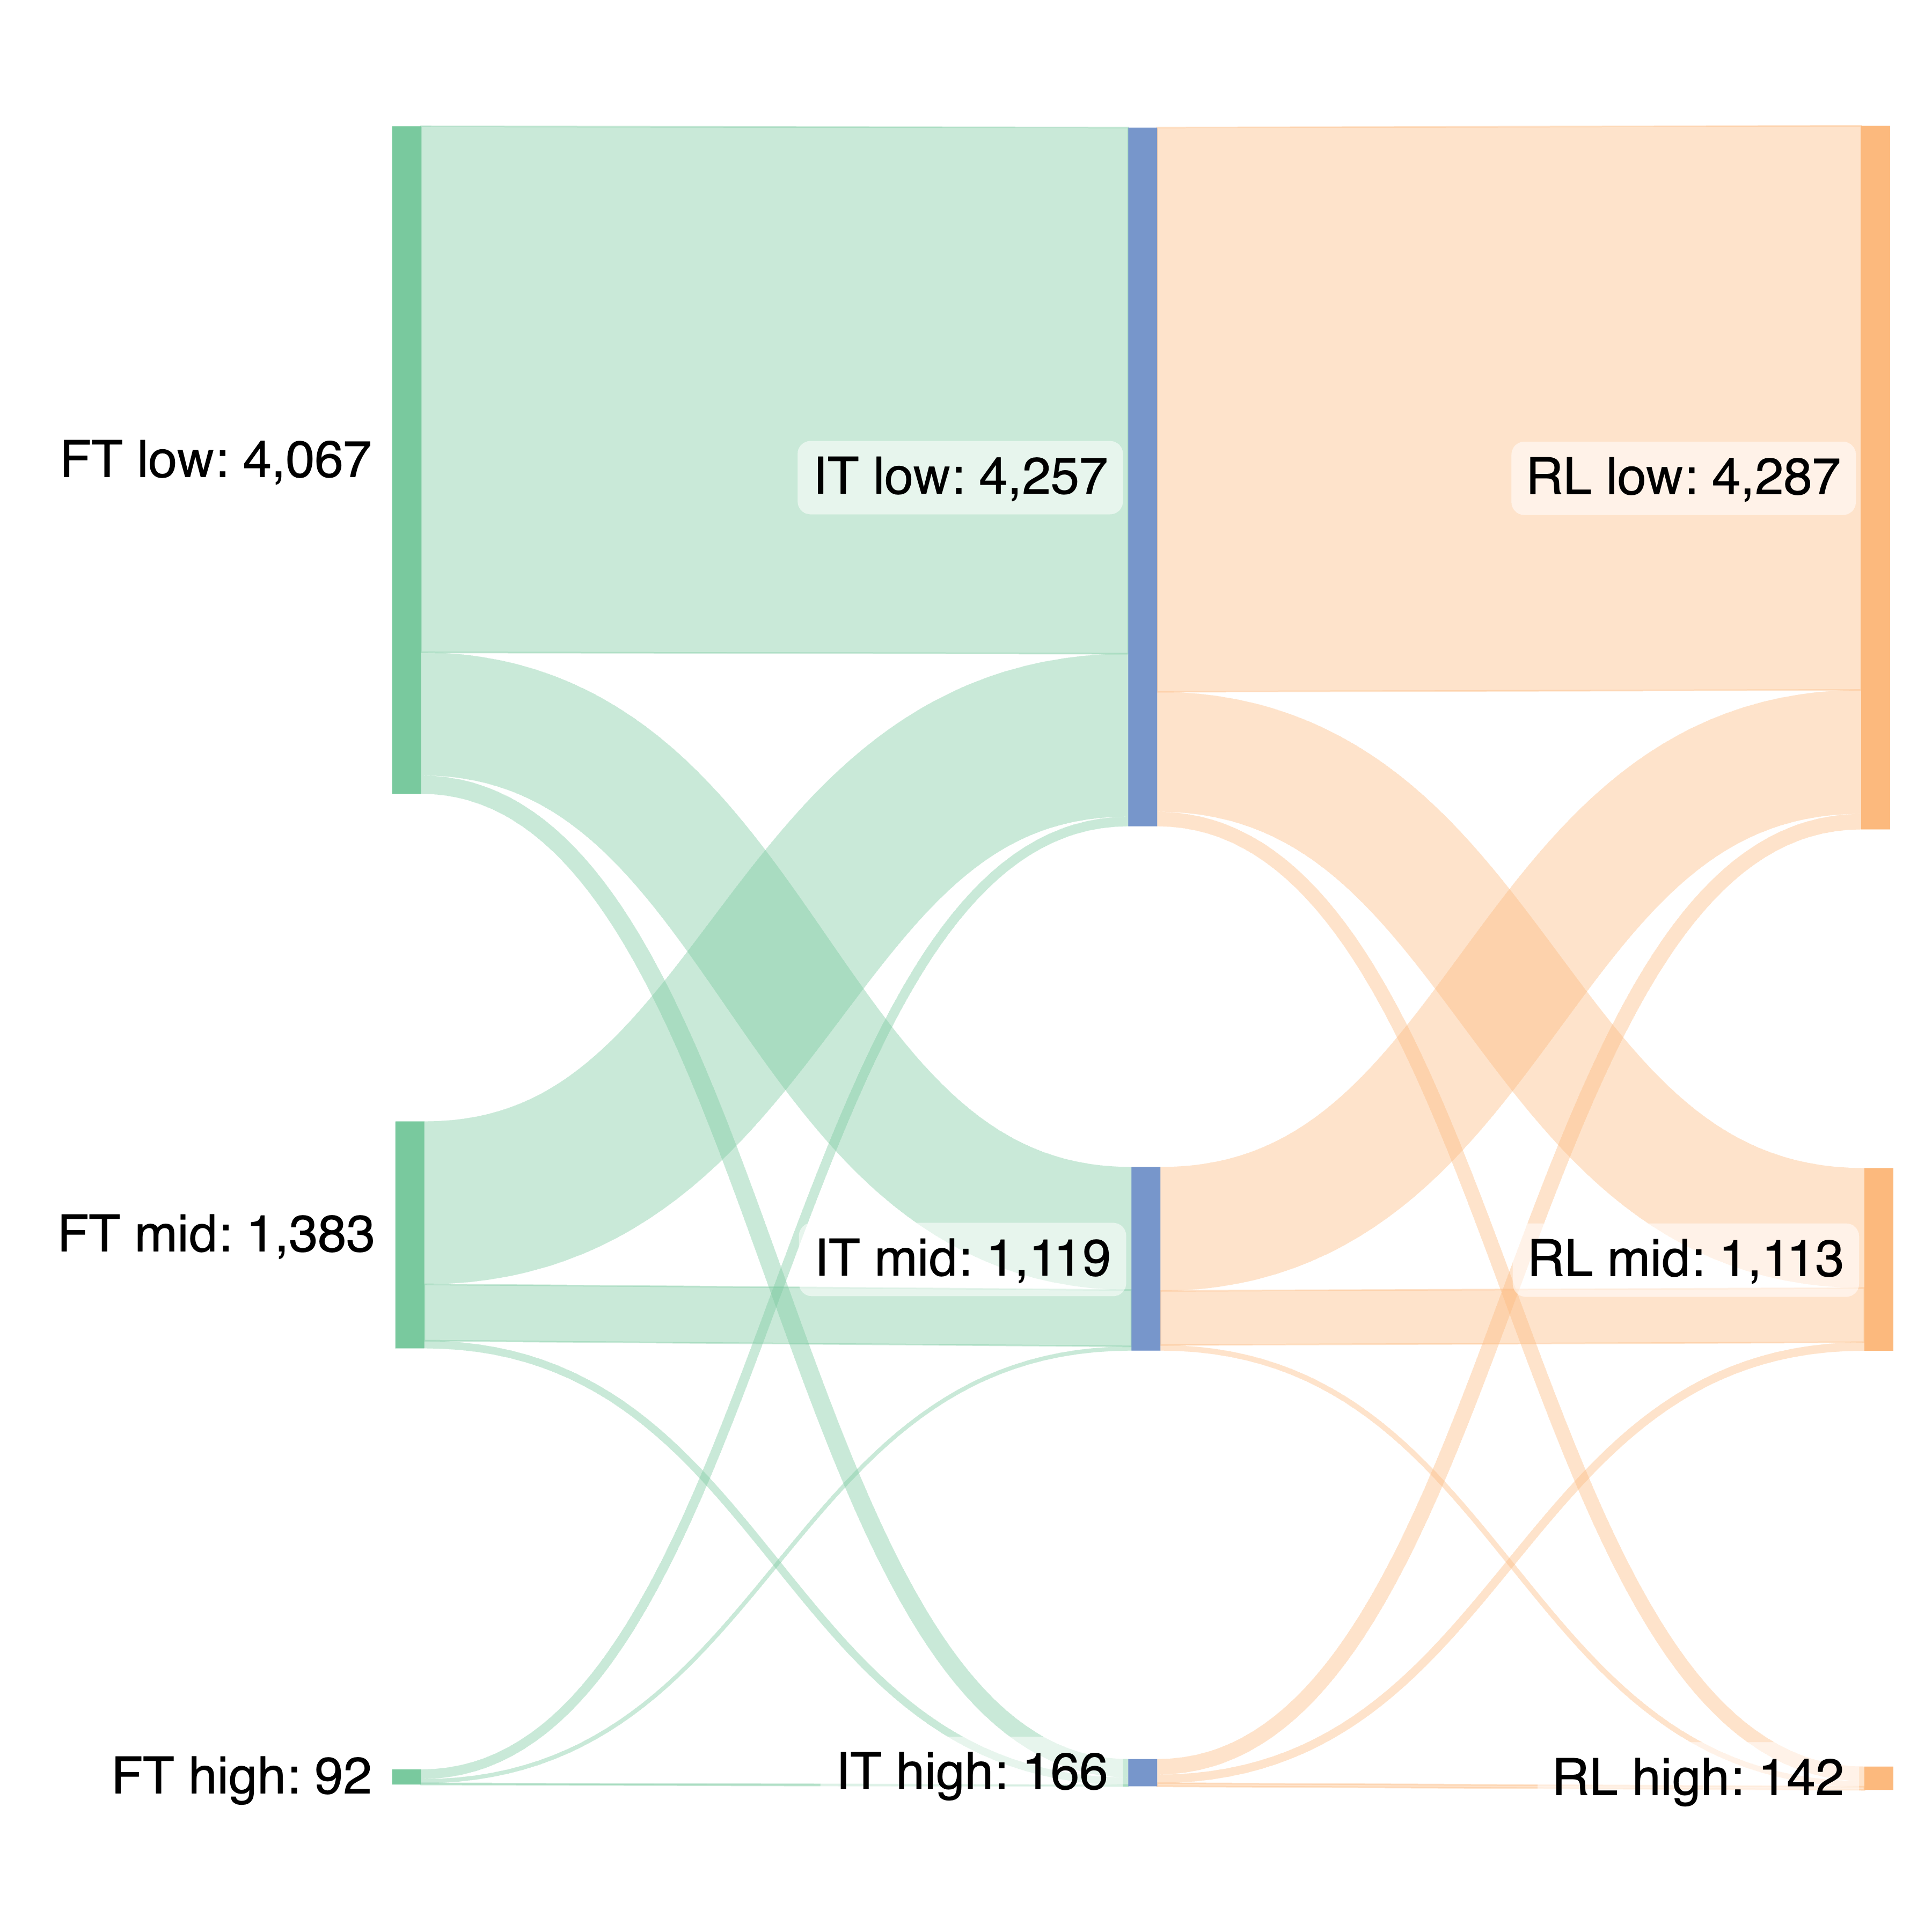
\includegraphics[width=.9\linewidth]{Figs/sankeymatic-falcon.png}
  \caption{Falcon 7B}
  \label{fig:sub2}
\end{subfigure}
\caption{Flow chart showing the shift of RTP instances for the different training types and models (\ref{fig:sub1}, \ref{fig:sub2}). Each column represents a type of training. Starting from the centre is the baseline (IT), going to the right it is possible to observe the shift towards the results given by training with Reinforcement Learning (RL) and, towards the left, the results of fine-tuning with counter-narrative (FT). The instances are divided into [low, mid, high] toxicity scores given by PerspectiveAPI, respectively [tox. lev $< 0.33$, $0.33 \leq$ tox. lev $\leq 0.66$, tox. lev $> 0.66$].}
\label{fig:flowchart}
\end{figure}



\section {Interpreting model behaviour}


A key part of the research project is to understand how the prompts given to the model are taken into account during the production of the output. This process allows for a more detailed analysis of how much the model relies on the prompt itself, the internal pre-training parameters and the tokens previously generated. It is important to analyze these aspects not only with regard to the study of the models themselves but also to understand how the post-training mechanisms used succeed or failed in changing these behaviours. By comparing metrics measured for the pre-trained models, then fine-tuned or trained with reinforcement learning, it is possible to identify where and how these changes occur, increasing the understanding of how mechanisms work in a procedure that by definition is considered to be black-box.

\begin{figure}
    \centering
    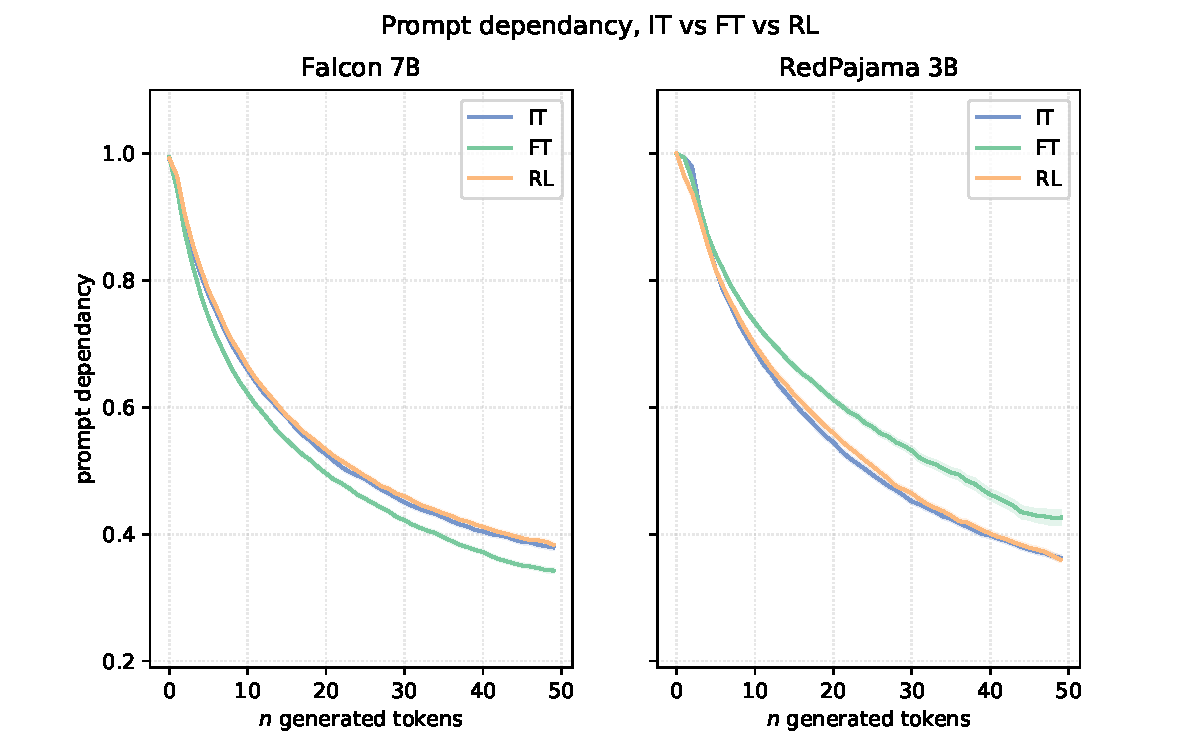
\includegraphics[width=\linewidth]{Figs/prompt-dependancy.pdf}
    \caption{Average prompt dependency for the first 50 tokens generated by the models. IT represents the baseline while FT and RL are the same models fine-tuned with counter-narrative or trained with reinforcement learning respectively.}
    \label{fig:prompt-dependancy}
\end{figure}

In figure \ref{fig:prompt-dependancy} it is possible to take a preliminary look at prompt dependence during model generation. Specifically, as tokens are generated, the dependence on the prompt (measured as a percentage between $0$ and $1$) drops, leading the model to generate tokens considering more and more of what it has previously generated in previous instants. By looking more closely, only the fine-tuned version of the model (FT) has a different drop rate if compared to the pre-trained baseline (IT) and the model trained with reinforcement learning (RL). Moreover, the drop rate pattern and shift for the fine-tuned version of Falcon 7B and RedPajama models do not seem to be equal: the fine-tuned version of Falcon 7B drops faster if compared to the fine-tuned version of RedPajama.


\paragraph{Shifts in toxicity following post-training techniques} With reference to the flow charts in figure \ref{fig:flowchart}, we aim to investigate how prompt dependency is influenced by the various classes of the different generations, based on the toxicity returned by PerspectiveAPI. As observed, for most prompts the detoxification process is effective, lowering the level of toxicity from \textit{high} to \textit{low}. However, this process also occurs, albeit in much smaller numbers, the other way around, i.e. with prompts that originally produced \textit{low} toxicity generations at baseline but which, after the post-training process (FR or RL), raised the toxicity of their generation to \textit{high}. There are also prompts which, on the other hand, have not undergone any shift as a result of the post-training technique deployed; prompts which at baseline (IT) led to toxic generations (\textit{high}) and which, after any post-training technique, lead to the same type of toxic generation are therefore of particular interest. The prompt dependencies of Falcon 7B and RedPajama 3B for these shifts are highlighted in Figures \ref{fig:falcon-shift} and \ref{fig:redpajama-shift} respectively.

\begin{figure}
    \centering
    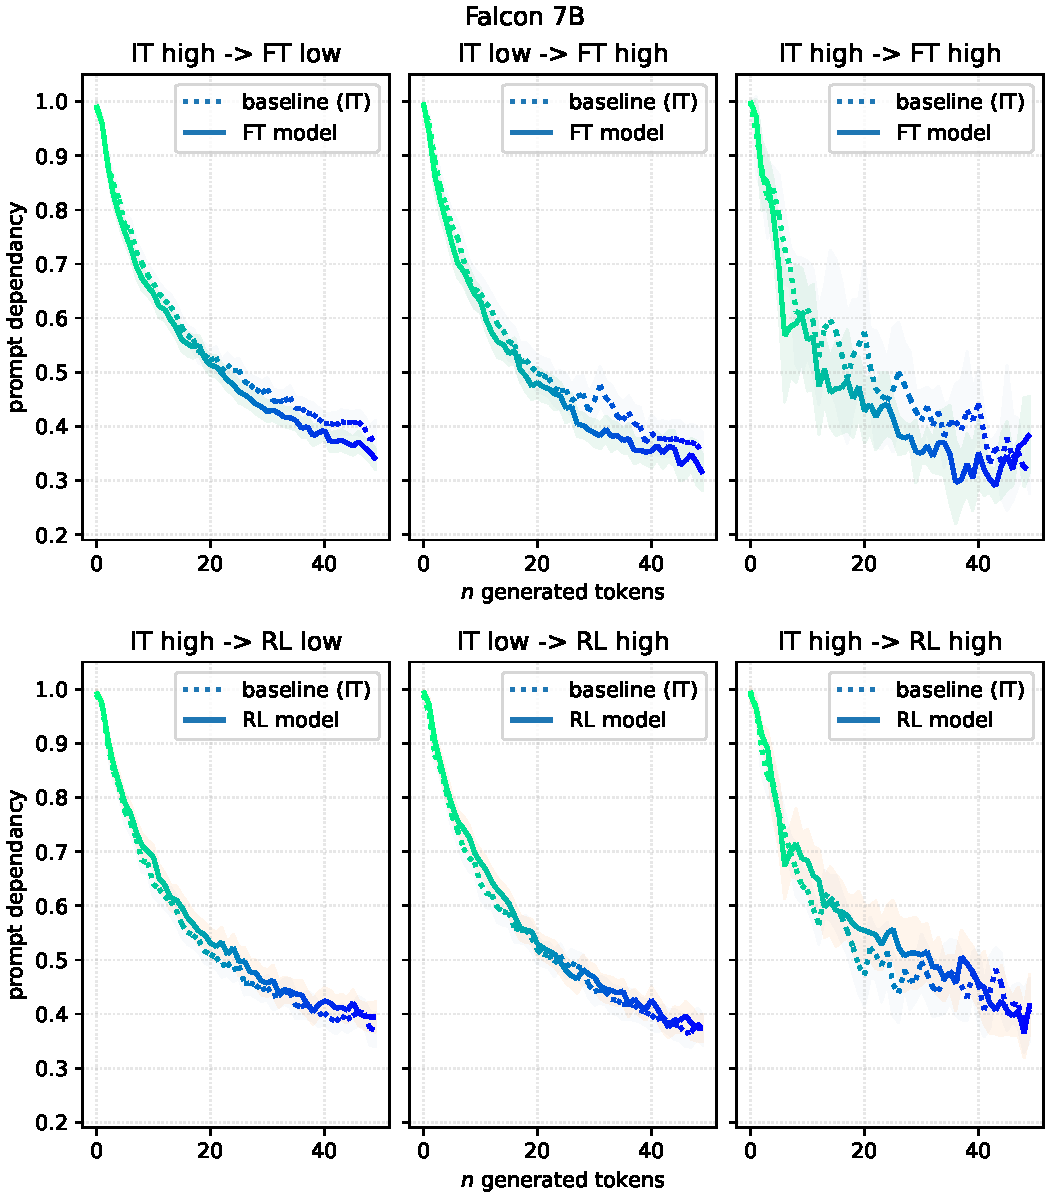
\includegraphics[width=0.9\linewidth]{Figs/falcon-shifts.pdf}
    \caption{Impact on prompt dependency during generation of the first 50 tokens for Falcon 7B model. The same prompts that belonged to a [high, low] toxicity class at baseline later became [high, low] toxicity class as a result of the post-training technique adopted (FT or RL). More specifically, the first column refers to the detoxification process (high to low toxicity), the second column to the inverse process, and the last column represents the toxic generations on which the post-training technique adopted had no impact.}
    \label{fig:falcon-shift}
\end{figure}

\begin{figure}
    \centering
    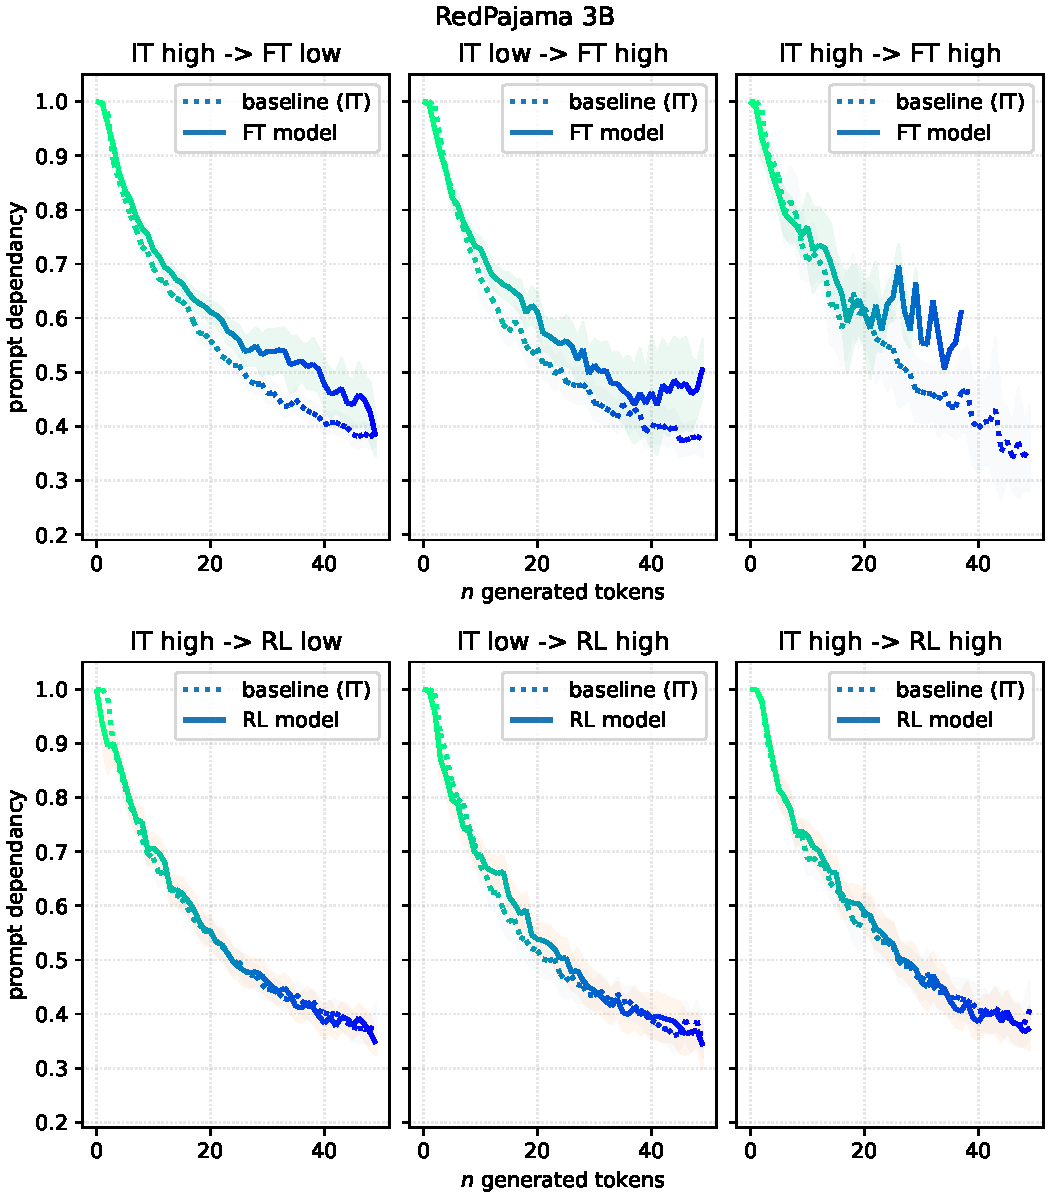
\includegraphics[width=0.9\linewidth]{Figs/redpajama-shifts.pdf}
    \caption{Impact on prompt dependency during generation of the first 50 tokens for RedPajama 3B model. The same prompts that belonged to a [high, low] toxicity class at baseline later became [high, low] toxicity class as a result of the post-training technique adopted (FT or RL). More specifically, the first column refers to the detoxification process (high to low toxicity), the second column to the inverse process, and the last column represents the toxic generations on which the post-training technique adopted had no impact.}
    \label{fig:redpajama-shift}
\end{figure}


For each model generation shift, the attributions on the prompt are reported for both the baseline (IT) and fine-tuned model with counter-narrative (FT) or reinforcement learning (RL), so that the attribution shift between the two can also be observed.

Starting from the case presented in Figure \ref{fig:falcon-shift}, regarding the largest model (Falcon 7B), it can be seen that, the dependence on prompts during generation, is slightly different between baseline and fine-tuned versions with both FT and RL. Looking in more detail it is interesting to note that the RL version, for all toxicity levels, has a higher prompt dependence than its FT counterpart, which is especially evident during the generation of the final tokens regardless of toxicity level. In general, FT seems to slightly lower the prompt dependence compared to the baseline, RL on the other hand seems to maintain the same pattern observed in the baseline. Considering the toxicity levels and their shifts, it is observed that, especially for prompts that produce highly toxic responses on both baseline and FT with counter-narrative (last column), although toxicity remains unchanged the model leans less on the prompt on average during generation. In contrast, the same behaviour is not observed in the case of standard RL-based detoxification where reliance on the prompt, even considering confidence intervals, remains almost the same.

On the other hand, regarding the smaller model (RedPajama 3B), with the same data presented in Figure \ref{fig:redpajama-shift}, more pronounced behaviours are observed regarding fine-tuning with counter-narrative (FT). In fact, in this case, the dependence on the prompt, in the generation phase, increases considerably compared to the baseline, a sign that the model looks much more at the prompt than at the generation it produces itself. This behaviour occurs for all toxicity levels and shifts represented, including the last column having both toxic generations. In general, even when analyzing the data qualitatively, smaller models tend to trust their generations much less, following behavioural patterns closer to the training process. However, the real reason for this remains unknown, allowing the formulation of new hypothesis based on the lower storage capacity during training due to the smaller presence of internal parameters in the model itself.

On the other hand, with regard to the post-training process with RL, no particular shifts on any level of toxicity appear to occur, symbolizing how further analysis is needed to understand how the process actually affected the behaviour of the model by lowering its average toxicity.




\subsection{Measure Language Models' uncertainty with interpretability} 
In order to better investigate the differences, not only looking at the prompt dependency of the model, by having the information on the attribution matrix $A$, it is possible to find out what level of information, and consequent uncertainty, arises from the attributions on the prompt. To measure this factor, entropy is generally used in information theory, more specifically Shannon entropy, based on a better representation of bits with two possible values. Specifically, given a discrete random variable $X$, distributed according to $p : x \in [0, 1]$ entropy is given by:

\begin{equation*}
    H (X) \coloneqq - \sum_{x \in X} p(x) \log p(x) = \mathbb{E}[- \log p(X)]
\end{equation*}

The $\log$ base can be chosen based on the entropy application, but it is generally set to 2 for computing measurements. Entropy measures the expected (i.e. average) amount of information needed to encode the outcome of a random trial. Thus, the more entropy there is, the more space will be needed to represent the possible outcomes of an observed variable. This concept can also be observed as a representation of \textit{uncertainty}. In this second interpretation, entropy is seen as a measure of how predictable a certain outcome is; if this should be unpredictable, i.e. with each event having a low probability of occurring, the outcome will be more \textit{uncertain}. In this specific case, therefore, the aim is to measure the unpredictability and \textit{uncertainty} of the generative model in relying on the prompt for the generation itself.


\begin{figure}
    \centering
    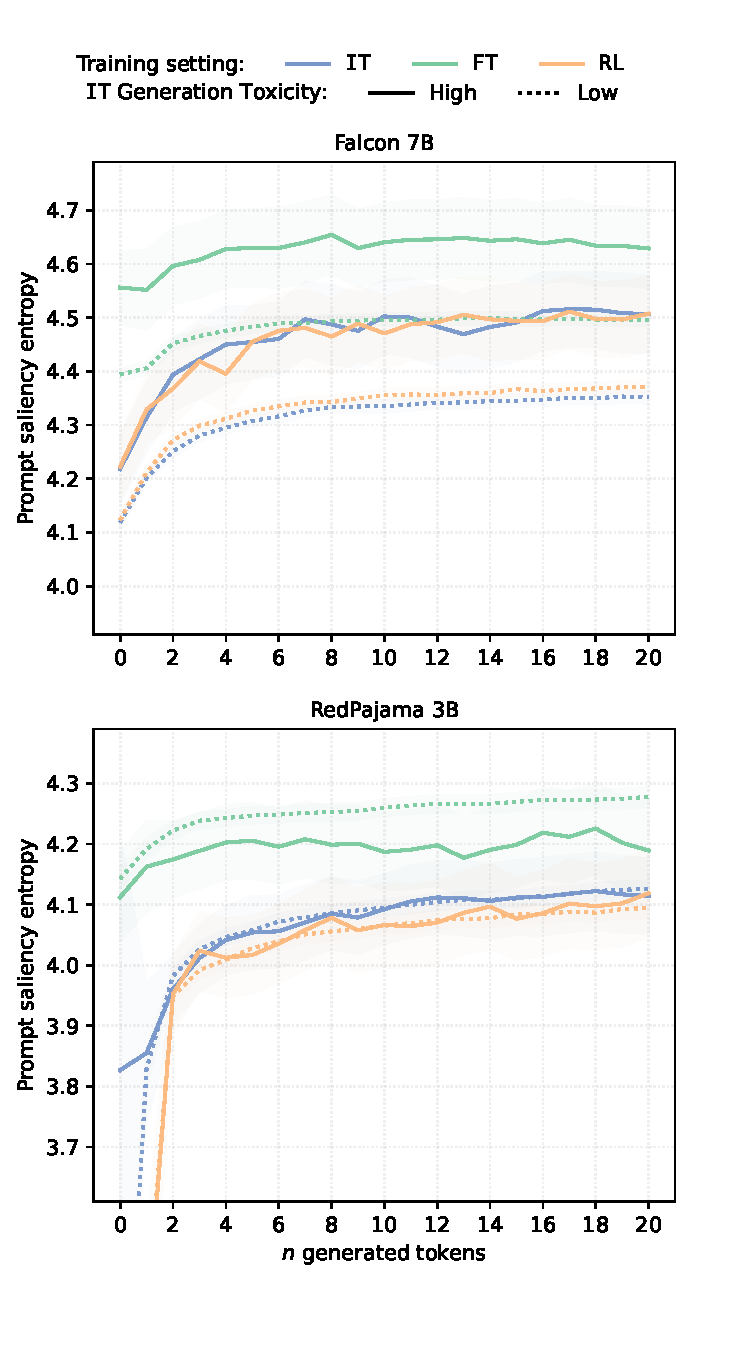
\includegraphics[width=0.8\linewidth]{Figs/prompt-dep-diff.pdf}
    \caption{Attribution entropy over prompt tokens throughout generation for Falcon and RedPajama models before (IT) and after (FT, RL) detoxification.}
    \label{fig:prompt-dep-diff}
\end{figure}


Throughout the generation of the text, it is possible to observe in figure \ref{fig:prompt-dep-diff} the distribution of entropy towards the prompt during the production of the output. Specifically, generations are also separated according to their level of toxicity reported by the baseline IT model. This step is performed to show how, in the toxic generations of the original model, fine-tune-based training with counter-narrative (FT) and Reinforcement-learning-based training (RL) changed the baseline behaviour in terms of reliance on the prompt. 

Looking at the results found, first for Falcon 7B then for RedPajama 3B, a pattern can be observed, where the FT model differs from the IT baseline and RL model. Interpreting the results, it can be seen that the fine-tuned model has more uncertainty in the generation, given the higher entropy, for all those prompts that led to toxic generations in the baseline model.

In general, it can be said that, on the same prompts that lead to toxic generation in the baseline model, fine-tuning with counter-narrative raises the entropy of attributions on the prompt. In other words, looking at the entropy calculation, the attribution scores are more evenly distributed on the prompt, compared to baseline and training with Reinforcement Learning.

This leads to considerations about the behaviour of the model towards the prompt: it is assumed that, in order to generate a counter-narrative, the model is inclined to look at the whole prompt instead of focusing exclusively on specific terms. It is therefore more important for the model to look at the whole prompt instead of just a few tokens, as is generally the case for generations measured from the baseline. Intuitively, this behaviour makes sense for generations that aim to counter what is said in the prompt, which would lead to toxic content. 

For training with Reinforcement Learning, on the other hand, this aspect is not observable. This is probably because, RLHF type approaches, certainly lead models to be less toxic (look at the results on model detoxification) but tend to limit their generations instead of pushing the model to understand what the prompt wants to communicate and possibly respond in agreement or disagreement.

By matching the results highlighted by the model interpretation with those obtained from the detoxification process of the models, it can be noted that the detoxification technique with higher performance (FT) obtained more evenly distributed attributions towards the prompt. This result, leads to interesting hypotheses about the detoxification process itself as a key part in improving existing pre-trained models. Indeed, the counter-narrative approach employed makes the models not only safer and less toxic but also improves their capacity to respond. Qualitatively, as previously pointed out in Table \ref{tab:ex-detox}, this leads to a better balance between helpfulness and harmlessness of the model but especially to an improvement measurable in quantitative terms through interpretability techniques.

Moreover, it is possible to make some considerations about the time trend in terms of model generations, i.e., the entropy trend on the attributions that the model makes during the next token prediction task. An interesting growth in entropy can also be observed for the initial tokens of generation. This, in agreement with what has been observed above, is directly related to the distribution of attribution values, which are probably concentrated more on tokens that are considered to be principal or of greater importance. This steep entropy increase, especially evident in the non-FT models, could indicate strong conditioning of the output that follows from specific terms used within the prompt.

In conclusion, it was possible to point out a common pattern between the two models under analysis that highlights how pushing LMs toward counter-narrative generations leads to new results in terms of attribution toward the prompt in use. In more general terms, this aspect turns out to be of fundamental importance, especially with regard to the possibility of generalizing phenomena within the model. Different behaviours of the model can highlight features otherwise difficult to identify through standard metrics, further giving an interpretation as to how the model reasons toward a given prompt or in a given context. As introduced in section \ref{chapter:SOTA} about the state of the art, currently, language models, are tested by measuring their potential toxicity by stimulating through specific prompts risky contexts within which to respond. An approach based instead on output interpretation would establish greater confidence in the model generation process, ensuring greater distinction of contexts and thus a more stable behaviour in given scenarios. The results highlighted here, together with red teaming processes already known in the literature, would ensure greater confidence in the proposed results, leading to generally more secure and reliable models.







